
\documentclass[conference]{IEEEtran}
\usepackage{amssymb}
\usepackage{amsmath}
\usepackage{bm} 
\usepackage{xspace}
\usepackage{algorithm}
\usepackage{algpseudocode}
\usepackage{varwidth}
\usepackage{threeparttable}
\usepackage{multirow,bigdelim} 
\usepackage{booktabs}
\usepackage{dsfont}
\usepackage{epsfig}
\usepackage{graphicx}
\usepackage{hyperref}
\usepackage{xspace}
\usepackage{color}
\usepackage{epstopdf}
\usepackage[font=footnotesize]{subfig}
\usepackage{chngpage}
\usepackage{subfig}
\usepackage{setspace}




\begin{document}

\title{\Large Learning from Sets}
%\author{Mohit Sharma~\thanks{University of Minnesota.}}
\date{}
\maketitle

\begin{abstract}
Existing item recommendation methods rely on the availability of the user’s
preferences on the items consumed in the past. Additionally, the performance
of these recommendation methods is proportional to the amount of information
available to the recommender system, i.e., the more availability of user’s
preferences on the items, the better the quality of the recommendations for
the user. However, it is not easy to elicit the user’s preferences on items to
improve the recommendations for the user, particularly when we have a large
number of items. In this paper, we propose a method in which we elicit the
user’s preference on a set of items rather than on the individual items that
constitute the set. We use this preference on the set to estimate the user’s
preference on the items that constitute the set. This method, compared to the
process in which the user has to provide sequentially his/her preference for
the individual items, can quickly gather the user’s preferences on a few sets
that span a large number of items. In the experiments on real-world data, we
show that the quality of recommendations generated from these sets is
comparable to the recommendations generated using the individual preference on
the items.
\end{abstract}

\section{Introduction}
%%!TEX root = paper.tex

Recommender systems are widely deployed in various domains e.g. music (iTunes),
movies (Netflix) and e-commerce (Amazon) to suggest relevant products to the users
based on their preferences. 

One of the key methods used by the recommender systems is the collaborative
filtering method, which uses the information from the previous transactions of 
the users and suggest relevant products to consume in the future. Generally, the collaborative
filtering consists of two approaches: the neighborhood - based approach and the
latent-factor models. In the neighborhood - based approach ~\cite{r30}, the similarities
between the items or the users are used to compute recommendations. While the
latent-factor models ~\cite{r4} transform the users and the items to the same
latent space where both of them are comparable to each other, the items closest
to the users in this space serve as the recommendations to the users.


An important requirement of these collaborative filtering methods is that the
user should indicate his/her preference over a certain number of items to
generate recommendations for future consumption. For existing users this is
not a significant problem, as these users have already consumed some items in the
past and will continue to provide information as they consume the items. 
However, this is a significant problem for the new user as there is no prior 
information available about their preferences and hence the recommender systems
fails to provide personalized recommendations to such users. These users are also
known as "cold-start" users.

To overcome this problem for a new user, most services deploying recommender 
systems elicit a user's preferences on a few popular items which the user may 
have consumed before. 
This process of eliciting the preferences of the users on the items is time
consuming as a user has to indicate his/her preferences on items one at a time.
Hence, the user may quit this preference elicitation process without completing
it, thus leading to poor initial recommendation performance for the user.

In this work, we present a method which elicits preferences of the user on a set of
items rather than rating those items individually in a sequence. This preference
on the set is used to estimate the preferences on the individual items that
constitute the set. Since a set can be composed of multiple items the  user 
can indicate his/her preference on a large
number of items by indicating his/her preference on a few sets of items.  
Hence, the time spent by a cold-start user to elicit his preferences in order to get
personalized recommendations is reduced significantly.


%TODO: Introduce model in simple words, like non-linear and linear and sigmoid add citatons

We make the following contributions: First, we propose various Learning from Set
models that enables estimation of the user's preference on the individual items.
Second, we illustrate the effectiveness of these models with experiments on the 
synthetic and the real datasets by comparing their performance with the state-of-the-art 
matrix factorization methods.


The rest of the paper is organized as follows. Section 2 introduces the
notations used in the paper. In Section 3, the relevant existing methods are
described. Section 4 presents the Learning from Set models. In Section 5,
details about evaluation methodology and dataset are provided. Sections 6
provides the results of the experimental evaluation. Finally, Section 7 gives
some concluding remarks.





\section{Notations and Definitions}
%%!TEX root = paper.tex
Throughout the paper, all vectors are column vectors and are represented by
bold lowercase letters (e.g., $\bm{u}$). Matrices are represented by upper
case letters (e.g., ${R,U,V}$).

The historical preference information is represented by a preference matrix $R$.
Each row in ${R}$ corresponds to a user and each column corresponds to an item. 
The entries of $R$ indicates  the users' preferences on the items. 
The preference given by the user $u$ for the item $i$ is represented by entry $r_{u,i}$ in $R$.  
The symbol $\tilde{r}_{u,i}$ represents the score predicted by the model for the actual
preference $r_{u,i}$.

Sets are represented with calligraphic letters. The set of items $\mathcal{S}$
has size $|S|$.





\section{Related Work}
%%!TEX root = paper.tex

\subsection{Collaborative Filtering}

Collaborative filtering is one of the widely used methods in the recommender
systems. It tries to estimate the rating on a user $u$ on item $i$ i.e.,
$\tilde{r}_{ui}$  based on the  partially observed user-item rating matrix $R
\in \mathcal{R}^{m \times n}$ for $m$ users and $n$ items. In order to generate
recommendations of new items, we need to estimate the unobserved entries of the
matrix $R$. The unobserved entries can be estimated by assuming the matrix $R$
to be of low-rank and completing the matrix $R$ by minimizing a squared loss:

%TODO: argmin (P,Q) equation, add citations

\begin{equation}
  (\tilde{P}, \tilde{Q}) = \arg \min_{P,Q} \sum_{(u,i)} ( R - [PQ^T]_{u,i})^2,
\end{equation}

where $P \in R^{m \times r}, Q \in R^{n \times r}$. The completed matrix
$\tilde{R} = \tilde{P} \tilde{Q}^T$
is used to serve the recommendation to the user for the items for which his
preferences were unknown in the original matrix $R$.







\section{The Movielens set ratings dataset}

%!TEX root = paper.tex

\subsection{Data collection}
Movielens\footnote{www.movielens.org} is a recommender system that utilizes collaborative filtering
algorithms to recommend movies to their users based
on their preferences.
We collected ratings from the Movielens users on certain sets of movies. These
sets were generated by selecting five movies from the movies that user has
already rated. There was no overlap among the sets presented to the user in a
session. The user can rate at most 50 such sets in a session. An example of
the questionnaire eliciting a user's rating on a set of movies is shown in the
Figure~\ref{fig:mlset}. The rating widget in the interface could be rated from 0 to 5 with a
precision of 0.5. For the purpose of data collection, we selected users who were active on the
Movielens since January 2015. The data was gathered from the user's responses to
the questionnaire from Feb 2016 to April 2016.


\begin{figure}[ht]
  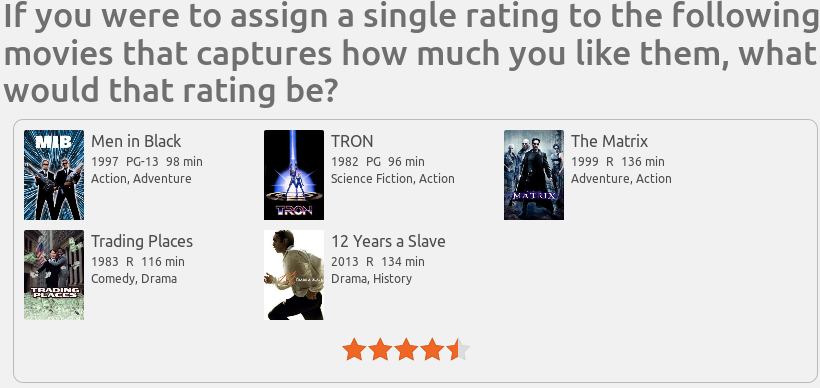
\includegraphics[scale=0.30]{figures/mlset.png}
  \caption{The interface used to elicit users' ratings on a set of movies.}
  \label{fig:mlset}
\end{figure}

\subsection {Data pre-processing}
Before processing the dataset, we removed users who have rated sets within a
time interval of less than one second to avoid users who might be guessing
the ratings at random. 



\subsection{Analysis of set ratings}
After data pre-processing step, we were left with ratings
from 854 users over 29,516  sets containing 12,549 items. 
Figure~\ref{fig:setratingdist} depicts
the distribution of the collected ratings. We also computed the mean rating of
each user and is shown in the Figure~\ref{fig:meanratingdist}.  

\begin{figure}[ht]
  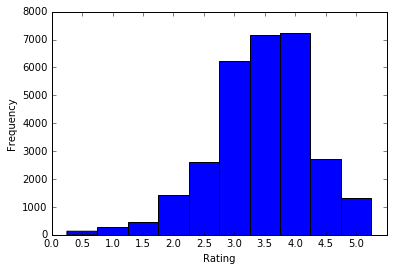
\includegraphics[scale=0.65]{figures/setratingdist.png}
  \caption{Ratings distribution.}
  \label{fig:setratingdist}
\end{figure}

\begin{figure}[ht]
  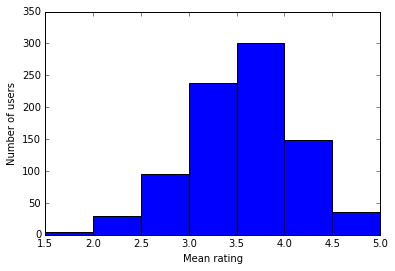
\includegraphics[scale=0.65]{figures/meanratingdist.png}
  \caption{The distribution of users' mean rating.}
  \label{fig:meanratingdist}
\end{figure}



The Figure~\ref{fig:usersetdist} shows the distribution of the number of sets rated by the user,
and we can see that roughly half of the users, i.e., 428 users have rated more
than 90\% of the sets, i.e., at least 45 sets in a session.

\begin{figure}[ht]
  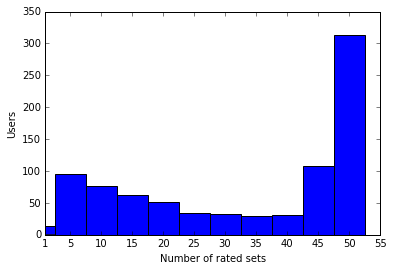
\includegraphics[scale=0.65]{figures/usersetdist.png}
  \caption{The distribution of number of sets rated by the users.}
  \label{fig:usersetdist}
\end{figure}

Since we know the actual rating of the users over the movies in the sets,
these ratings can help us understand the users' behavior when assigning a single
rating to a set of movies. To this end, we computed the deviation of the 
rating assigned by a user to the set
from the average of the user's  ratings of the items constituting the set. To
calculate this deviation we computed the Root Mean Square Error (RMSE) between
the ratings assigned to the sets and the average of the user-item ratings in
the sets. As can be seen in the Table~\ref{table:sets_rmse_table}, this RMSE
over all the sets is 0.597. Subsequently, we looked at the fraction of sets that are
rated below the average of the ratings of the items in the set. We refer to
these sets as the under-rated sets. Similarly, the over-rated sets are
those sets that are rated above the average of the ratings of the items in the
set.We used a margin of 0.5 while identifying these sets, i.e., sets rated
within the margin of 0.5 of their average rating were considered neither as
over-rated or under-rated sets.

%TODO:statistical significance of lower RMSE
The Table~\ref{table:sets_rmse_table} shows that the majority of the sets were neither over-rated or
under-rated and had a significantly lower RMSE of 0.241 when compared against
under-rated or over-rated sets. Further, we selected users who have rated at
least 50 sets and computed the fraction of under-rated and over-rated sets.
As can be seen from the Figure~\ref{fig:underrated}, some users tend to over-rate or under-rate sets
and by the Kolmogorov-Smirnov 2 sample test this behavior was found to be
statistically different (P-value $<$ 1e-16) from that of random.

\begin{table}[t]
  \centering
  \caption{RMSEs across different type of sets.}
  \label{table:sets_rmse_table}
  \begin{tabular}{|l|c|c|c|}
    \hline
    Type
    &\multicolumn{1}{|p{2cm}|}{\centering \% of Sets}
    &\multicolumn{1}{|p{2cm}|}{\centering Number of Sets}
    &\multicolumn{1}{|p{1cm}|}{\centering RMSE} \\
    \hline
    Over-rated  & 17.68 & 5,220  & 0.962 \\
    Under-rated & 22.26 & 6,571  & 0.810 \\
        Neither & 60.05 & 17,725  & 0.241 \\
    \hline
    All & 100   & 29,516 & 0.597 \\
    \hline
  \end{tabular}
\end{table}


\begin{figure*}[ht]
  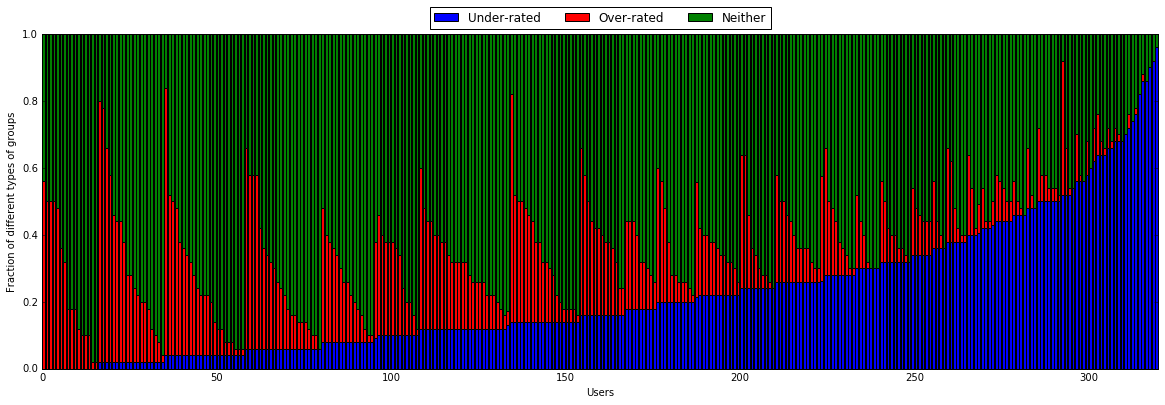
\includegraphics[scale=0.45]{figures/underrated.png}
  \caption{Fraction of different types of sets across users.}
  \label{fig:underrated}
\end{figure*}


Further, we examined the effect of diversity of the items' rating in the set,
i.e., whether the presence of movies with varying degree of ratings has any
effect on the rating assigned by the user to the set. For each set, we
computed the difference between the item's rating and the average of the ratings
in the set. We defined set-deviation as the square root of the mean of this
difference of the items' ratings in the set. The sets having deviation
greater than 1.0 were characterized as "Diverse" sets and rest as
"Non-Diverse" sets. Following this characterization in the dataset, nearly 20\%
of the sets are diverse sets having RMSE of 0.725 while remaining sets
have lower RMSE of 0.559.  This indicates that user seems to under-rate or
over-rate diverse sets more in comparison to non-diverse sets.


We also investigated whether the presence of movies that are rated recently or
that are rated in the past has an effect on the rating assigned to the set.
To this end, for each set we computed the difference between the timestamp of
the earliest rating and 2016, i.e. when the users were asked to rate the sets.
Interestingly, the under-rated sets contained ratings that were provided on
average 1,800 days,i.e., five years before the survey while remaining sets
contained ratings that were provided approximately 1,450 days, i.e.,
four years before the survey. This difference among the sets was found to be
statistically significant by T-test, i.e. P-value $<$ 1e-16. This suggests that
the user's preference for a movie in a set appears to decay temporally leading
to under-rating of the set containing that movie.




\section{Methods}
%%!TEX root = paper.tex

To estimate the preferences on individual items from the preference of the user on the
sets, we need to understand how the user rate a given set of items. A user may
rate a set of items by considering each item in the set or may chose to rate
the set of the items based on few but majority of the items in the set.

In the first case, when a user consider all the items in the set before 
assigning a rating to a set then we can safely assume that the user most likely
gives the set an average score of his preferences for all the items that constitutes 
the set. Under this assumption the estimated rating of the user $u$ on a 
set $S$ is given by: 

\begin{equation} \label{avgSetEq}
  \begin{split}
    \tilde{r}^{avg}_{us} &= \frac{1}{|S|} \sum_{i \in \mathcal{S}} r_{u,i},
  \end{split}
\end{equation}

where $\mathcal{S}$ denotes the set containing the items and $r_{u,i}$ is the
preference score of the user $u$ on the item $i$ .

Similarly, when a user considers only a few but the majority of the items in
the set $\mathcal{S}$ then the user's estimated rating on the set $\mathcal{S}$ is given by:

\begin{equation} \label{majSetEq}
  \begin{split}
    \tilde{r}^{maj}_{us} &= \frac{1}{|\mathcal{S}_{maj}|} \sum_{i \in
    \mathcal{S}_{maj}} r_{u,i},
  \end{split}
\end{equation}

where $\mathcal{S}_maj$ contains the majority of the top rated items in the set 
$\mathcal{S}$.


Assuming that the original user-item preference matrix $R$ is low-rank, we can write
the estimated preference of the user $u$ for the item $i$ as follow:

\begin{equation} 
  \begin{split}
    \tilde{r}_{ui} &= p_u^Tq_i, 
  \end{split}
\end{equation}

where, $k$ is the rank of the matrix $R$, $p_u \in \mathcal{R}^k$ and $q_i \in \mathcal{R}^K$ denotes the latent factor of the user $u$ and the item $i$ respectively.  

Following the low-rank assumption, we can rewrite the estimated score of the 
user $u$ for a set $\mathcal{S}$ in equations \ref{avgSetEq} and \ref{majSetEq} as follow:

\begin{equation} \label{avgSetLoEq}
  \begin{split}
    \tilde{r}^{avg}_{us} &= \frac{1}{|S|} \sum_{i \in \mathcal{S}} p_u^Tq_i,
  \end{split}
\end{equation}


\begin{equation} \label{majSetLoEq}
  \begin{split}
    \tilde{r}^{maj}_{us} &= \frac{1}{|\mathcal{S}_{maj}|} \sum_{i \in
    \mathcal{S}_{maj}} p_u^Tq_i,
  \end{split}
\end{equation}


\subsection{Learning from Set Model}
The learning from set model is parameterized by $\Theta=[P, Q]$, where the
matrices $P$ and $Q$ contains the latent factors of the users and the items
respectively. The model parameters are estimated by minimizing the squared error
loss function, given by

%
\begin{equation} \label{eq_rmse}
  \mathcal{L}_{rmse}(\Theta) \equiv \sum_{u \in U} \sum_{\substack{s \in
  \mathcal{R}_{us}}} (\tilde{r}_{us} - r_{us})^2,
\end{equation}
%

%TODO: need to add better connection to majority or average assumption

where $\mathcal{R}_{us}$ contains all the sets preferred by the user $u$,
$r_{us}$ is the original rating and $\tilde{r}_{us}$ is the estimated rating of
the user $u$ on the set $s$. The estimated rating $\tilde{r}_{us}$ can be
computed as per equation \ref{avgSetLoEq} or \ref{majSetLoEq} depending on
whether the average or the majority assumption is used to estimate the rating of 
the user $u$ on the set $s$. 

To control model complexity, we add regularization of the model parameters
thereby leading to an optimization process of the following form:

%
\begin{equation} \label{eq_obj}
  \min_{P, Q} \sum_{u \in U} \sum_{\substack{s \in \mathcal{R}_{us}}} (\tilde{r}_{us} - r_{us})^2  + \lambda (\|P\|_F^2 + \|Q\|_F^2),
\end{equation}
%

where $\lambda$ is the regularization parameter.

%TODO: need to add better connection to majority or average assumption

The optimization problem of equation \ref{eq_obj} is solved by stochastic
gradient descent algorithm for the average assumption and stochastic
sub-gradient descent algorithm for the majority assumption.

%TODO: add pseudo-code algorithm
%TODO: add sub-gradient details and why it is needed




\section{Experimental Evaluation}
%\input{experiments.tex}

\section{Results and Discussion}
%\input{results.tex}

\section{Conclusion}
%\input{conclusion.tex}

%\bibliography{refs}{}
%\bibliographystyle{plain}

\end{document}



